\documentclass[a4paper,11pt]{article}

\usepackage[utf8]{inputenc}
\usepackage{amsmath,amssymb,graphicx,natbib,float,xcolor,geometry,mathptmx}

%%%% ---- Formatting ---- %%%%

% margins
%\geometry{a4paper, top=40mm, right=25.4mm, bottom = 25.4mm, left = 25.4mm}
\geometry{a4paper, top=25.4mm, right=25.4mm, bottom = 25.4mm, left = 25.4mm,
  footnotesep=20pt}

% links
\usepackage[pdfusetitle]{hyperref}
\hypersetup{hidelinks,colorlinks,urlcolor=[rgb]{0,0,1},citecolor=blue}

% paragraph formatting
%\setlength{\parskip}{12pt plus 0.2ex minus 0.2ex}
%\setlength{\parindent}{0pt}

% figure captions
\usepackage[font=small,labelfont=bf,margin=10pt]{caption}

% define keywords, title page and document properties
\makeatletter
  
  % define keywords variable
  \def\@keywords{}
  \newcommand{\keywords}[1]{
    \def\@keywords{#1}
  }

  % make title page
  \def\@maketitle{%
  \newpage
  \null
  {\centering
  \let \footnote \thanks
    {\Large \bfseries \@title \par}%
    %\vskip -4pt%
    \vskip 8pt%
    {\it \@author \par}%
  \par}
  %\vskip 12pt
  \vskip 8pt
 	\underline{keywords}: \@keywords
  }

%  % add info to pdf metadata
%  \hypersetup{pdftitle={\@title},pdfauthor={\@author}}

\makeatother

% change section heading
\makeatletter
\renewcommand\section{\@startsection {section}{1}{\z@}%
                                   %{36pt}%
                                   {12pt \@plus .5pt}%
                                   %{0.5pt \@plus.5pt}%
                                   {4pt \@plus.5pt}%
                                   {\centering\normalfont\bfseries}}
\makeatother


% bibliography
\bibliographystyle{plainnat}
\setcitestyle{authoryear}

% Put figures and text together
\def\textfraction{0.01}
\def\topfraction{0.99}
\def\dbltopfraction{0.99}
\def\bottomfraction{0.99}
\def\floatpagefraction{0.99}
\def\dblfloatpagefraction{0.99}
\def\dbltopnumber{100}



%%%% ---- Abstract Properties ---- %%%%


\title{Efficient Origami Construction of Orthogonal Terrains \\
using Cross-Section Evolution}
\author{Amartya Shankha Biswas, Erik D. Demaine, 
and Jason S. Ku}
\keywords{cross sections, orthogonal terrains, time evolution}


%%%% ---- Start Document ---- %%%%

\begin{document}

\maketitle


\section*{Abstract}

Many algorithms and universality results exist for producing parameterized
families of origami structures, but few are provably efficient, i.e. provide
constructions from a paper having dimensions within a low constant factor of an
optimal construction. At 5OSME, \cite{MazeFolding_Origami5} presented a
efficient construction for folding orthogonal mazes which is computable in
polynomial time. Origamizer presented in \cite{Origamizer_SoCG2017} constructs
foldings corresponding to general polyhedral surfaces, but does not provide any
bound on the efficiency of the constructions. On the other hand, TreeMaker from
~\cite{Lang} produces efficient crease patterns to fold uniaxial bases, but may
require exponential time to to find an efficient solution. 

In this paper, we present an algorithm for efficiently producing an origami
folding that corresponds to an input {\bf orthogonal terrain} with arbitrary
rational extrusion heights. A folding corresponds to an orthogonal terrain if
the folding covers every point on the terrain, but no point on the folding
exists above the terrain. This result improves an algorithm,
\cite{BoxPleating_Origami5} also presented at 5OSME, applicable to a more
general class of inputs, providing a universal construction to fold general
orthogonal polyhedra, though the construction is less inefficient than our
construction applied to orthogonal terrains. Our construction approach follows
three steps: 

\vspace{-0.2pc} 
\begin{enumerate} 
\item decompose the orthogonal terrain into strips that are constant along one
dimension; 
\item cover the strips efficiently using rectangular strips of paper; and 
\item stitch the strips together along matching boundaries. 
\end{enumerate}
\vspace{-0.2pc}

In order to better communicate the algorithm and the final folded state
produced, we also introduce a new {\bf cross-section evolution} representation
of a folded isometry: a straight line is swept across the crease pattern of a
folded surface, and we keep track of how the folding of the line evolves as a
cross-section of the folded surface. The propagation of the cross-section
between crease pattern vertices is uniquely determined by the initial
orientation of the cross-section, so the folded isometry can be constructed by
sweeping the line and locally modifying the cross-section when crossing crease
pattern vertices during propagation. This representation not only simplifies the
description of the 3D folded isometries constructed, but also provides a simpler
framework to argue that the folded state does not self intersect, by propagating
planar cross-sections monotonically along a single direction. We then
show that our construction's efficiency is within a small constant factor of
any folding with optimal efficiency.

% Decrease the space between bibliography items, without changing the first.
\let\realbibitem=\bibitem
\def\smallbibitem{\par \vspace{-1.2ex}\realbibitem}
\def\bibitem{\let\bibitem=\smallbibitem \realbibitem}

{
\small
\bibliography{extrude}

}

\begin{figure}
  \centering
  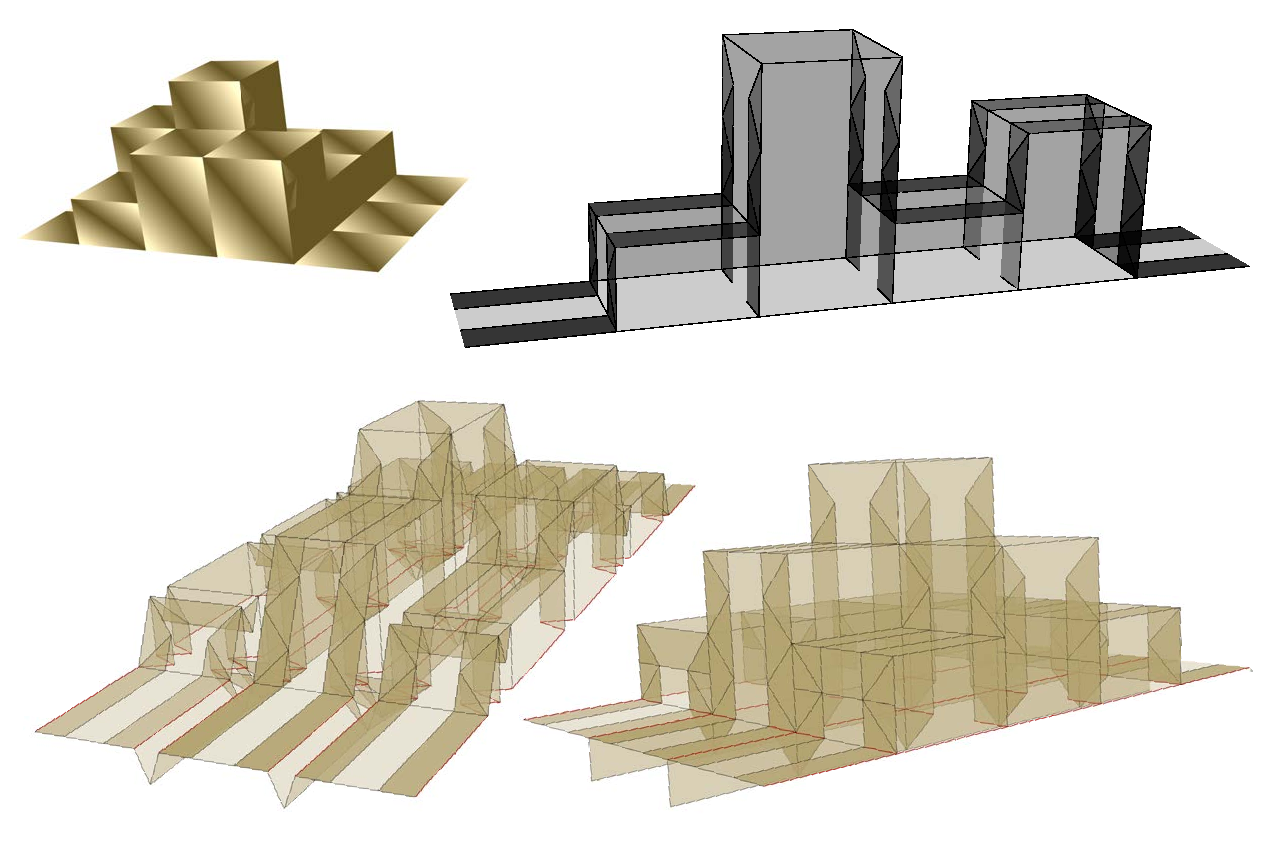
\includegraphics[width=\linewidth]{Figures/fig1sm.pdf}
  \caption{The construction progression a folding corresponding to an input
orthogonal terrain [top left]. We split the terrain into sections that are
constant along one direction, cover each strip with a rectangular strip [top
right], and then recombine the sections [bottom]. }
 \label{fig:extrude}
\end{figure}
\begin{figure}
  \centering
  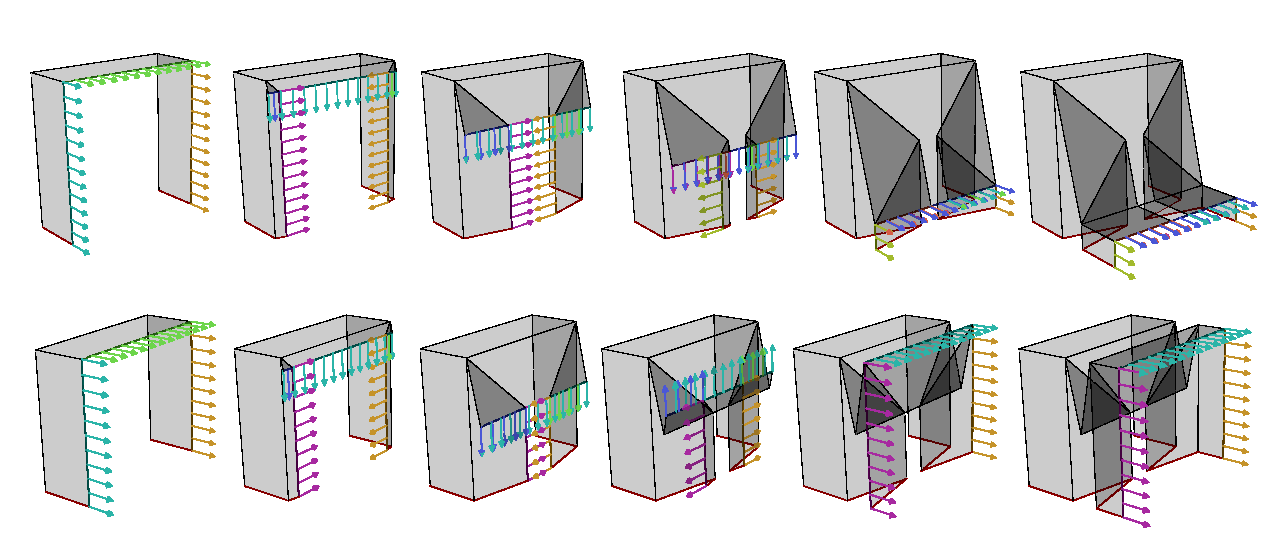
\includegraphics[width=\linewidth]{Figures/fig2sm.pdf}
  \caption{Snapshots of a cross-section evolution for two gadgets used to
construct orthogonal terrains. The sequence on top shows a level-shifting gadget
that changes the height of a section via the use of auxiliary pleats to tuck 
away excess paper. The sequence on the bottom shows a paper-absorbing gadget
that allows adjacent sections of paper that will later be attached together to
stay in sync with each other. }
 \label{fig:extrude}
\end{figure}


\end{document}
